% two-column draft
\documentclass[10pt,twocolumn]{IEEEtran}
\usepackage{setspace}

\singlespacing

\usepackage{cite}
\usepackage{amsthm}
\usepackage{amsmath,amssymb}
\usepackage[type1]{libertine}
\usepackage[libertine]{newtxmath}

% Make parantheses more round
\DeclareSymbolFont{largesymbols}{OMX}{cmex}{m}{n}
\DeclareMathSymbol{\intop}{\mathop}{largesymbols}{"52}
\DeclareMathSymbol{\sumop}{\mathop}{largesymbols}{"50}
\DeclareMathSymbol{\sqrtop}{\mathop}{largesymbols}{"70}
\usepackage{bm}
\allowdisplaybreaks
\renewcommand{\qedsymbol}{$\blacksquare$}
\usepackage{subfigure}

\usepackage{algorithmic}
\usepackage{graphicx}
\usepackage{textcomp}
\usepackage{xcolor}
\usepackage{hyperref}
\usepackage{cleveref}
\usepackage{commath}
\usepackage{optidef}
\usepackage{orcidlink}
\usepackage{lipsum}
\usepackage{stfloats}
\usepackage{tabularx}

\newtheorem{theorem}{Theorem}
\newtheorem{lemma}{Lemma}
\newtheorem{corollary}{Corollary}
\newtheorem{proposition}{Proposition}
\creflabelformat{lemma}{#2\textbf{#1}#3}
\creflabelformat{theorem}{#2\textbf{#1}#3}
\creflabelformat{corollary}{#2\textbf{#1}#3}
\creflabelformat{proposition}{#2\textbf{#1}#3}
\crefname{lemma}{\textbf{Lemma}}{\textbf{Lemmas}}
\crefname{theorem}{\textbf{Theorem}}{\textbf{Theorems}}
\crefname{corollary}{\textbf{Corollary}}{\textbf{Corollaries}}
\crefname{proposition}{\textbf{Proposition}}{\textbf{Propositions}}
\crefname{section}{Section}{Sections}
\crefname{figure}{Fig.}{Figs.}

\setlength{\tabcolsep}{10pt}
\renewcommand{\arraystretch}{1.45}

\newcommand\nnfootnote[1]{%
  \begin{NoHyper}
  \renewcommand\thefootnote{}\footnote{#1}%
  \addtocounter{footnote}{-1}%
  \end{NoHyper}
}

\def\BibTeX{{\rm B\kern-.05em{\sc i\kern-.025em b}\kern-.08em
    T\kern-.1667em\lower.7ex\hbox{E}\kern-.125emX}}

\begin{document}

\IEEEaftertitletext{\vspace{-1.5\baselineskip}}
\title{\huge{AeCC: Autoencoders for Compressed Communication}}
\author{Muhammad~Umer{~\orcidlink{0009-0001-8751-6100}}
and~Muhammad~Ahmed~Mohsin{~\orcidlink{0009-0005-2766-0345}}\\
{School of Electrical Engineering and Computer Science (SEECS), NUST, Pakistan}\\
{Email: \{mumer.bee20seecs, mmohsin.bee20seecs\}@seecs.edu.pk}\\
{CMS ID: 345834,~333060}
}

\makeatletter
\patchcmd{\@maketitle}
{\addvspace{0.5\baselineskip}\egroup}
{\addvspace{0\baselineskip}\egroup}
{}
{}

\makeatother
\maketitle
\begin{abstract}This project report presents a novel approach to image transmission using Vision Transformer (ViT) architecture and wireless communication principles. The methodology involves the division of input images into patches, subsequently fed into the ViT model. Leveraging the attention layer mechanisms of ViT, essential spatial information is extracted and encoded into a latent space. The latent space simulates a wireless communication channel, where Rayleigh noise is introduced to the features. The noisy features are then decoded at the output using a decoder, which itself is implemented as a Vision Transformer. The experimental results showcase the effectiveness of this hybrid framework, demonstrating its potential application in image transmission scenarios with inherent noise and communication channel modeling.

\end{abstract}

\begin{IEEEkeywords}
    Vision transformer, autoencoder, image compression, communication.
\end{IEEEkeywords}

\section{Introduction}
\IEEEPARstart{T}{he} rapid evolution of deep learning architectures has significantly impacted various domains, particularly in the field of computer vision and image processing. Among these, Convolutional Neural Networks (CNNs) have traditionally held a dominant position for their effectiveness in handling spatial hierarchies and local feature extraction. However, with the advent of Vision Transformer (ViT) architectures, a paradigm shift has occurred, redefining the way we approach image processing tasks \cite{khan2019robust}.

Unlike CNNs, ViTs exhibit a distinctive capability in understanding and processing global spatial information. The self-attention mechanisms embedded within ViTs enable them to capture long-range dependencies in an image, allowing for a holistic understanding of the content. This global perspective stands in contrast to the local focus of CNNs, which primarily extract features based on local receptive fields \cite{letizia2021capacity}.

The unique characteristics of ViTs make them particularly suitable for tasks that involve compression and feature extraction for latent spaces \cite{chandar2021communication}. In scenarios where the efficient encoding of spatial information is crucial, ViTs showcase a superior ability to compress information globally, leading to more effective representations.

Motivated by this advantage, our project explores the utilization of ViTs as autoencoders in an image transmission framework. The process involves dividing the input image into patches and passing them through a ViT. The ViT's attention mechanisms focus on crucial spatial information, effectively compressing and extracting features for the latent space. This latent space is then modeled as a wireless communication channel, and to simulate the noise inherent in non-line-of-sight (NLOS) channels, Rayleigh noise is introduced to the features \ref{perera2018ship}.

The introduction of Rayleigh noise serves to mimic the challenges encountered in wireless communication channels, allowing for a more realistic evaluation of the model's robustness and performance \cite{zebang2019densely}. Subsequently, the features embedded with Rayleigh noise are decoded at the output using a decoder, which is once again implemented as a ViT. This decoding process aims to mitigate the introduced noise, reconstructing the original image from the latent space \cite{letizia2020capacity}.

In this project, we aim to showcase the efficacy of ViTs as autoencoders for image transmission tasks, highlighting their unique ability to globally compress and extract features \cite{zhang2019optimally}. By incorporating Rayleigh noise and employing ViTs at both encoding and decoding stages, we anticipate significant insights into the performance of such models in wireless communication scenarios with non-line-of-sight channels. Through this exploration, we seek to contribute to the growing body of knowledge on leveraging advanced deep learning architectures for robust and efficient image transmission.

\section{Literature Review}
The rapid advancements in deep learning architectures, particularly Convolutional Neural Networks (CNNs) and Vision Transformers (ViTs), have significantly impacted various domains, including computer vision, image processing, and wireless communication. In this research, we focus on leveraging ViTs' unique capabilities for image transmission in non-line-of-sight (NLOS) wireless communication channels. To contextualize our work, we present a comprehensive literature review encompassing relevant aspects of CNNs, ViTs, image compression, and channel modeling for NLOS transmissions.

CNNs have traditionally dominated image compression and transmission tasks due to their effectiveness in extracting local features and exploiting spatial hierarchies. Early works like \cite{cheng2018deep} employed autoencoders with convolutional layers to achieve lossless compression, while \cite{saber2022list} explored the use of CNNs for channel coding and denoising in image transmission over noisy channels. However, CNNs primarily focus on local receptive fields, limiting their ability to capture long-range dependencies and global context within an image.

The emergence of ViTs marked a paradigm shift in image processing by introducing self-attention mechanisms, enabling them to capture long-range dependencies and understand global spatial information effectively. Unlike CNNs, ViTs process the entire image in its entirety, allowing them to learn richer representations and contextual relationships between different image regions. This advantage makes ViTs particularly suitable for tasks requiring strong global feature extraction and compression, such as image transmission through bandwidth-limited NLOS channels.

While ViTs' potential for image compression and transmission has been recognized, applying them in NLOS scenarios is an emerging research area. Recent works like [3] investigated the use of ViTs for image compression, achieving competitive results compared to CNN-based methods. However, limited research explores the specific application of ViTs for image transmission and reconstruction in NLOS channels.

Accurately modeling the transmission channel is crucial for evaluating the performance of image transmission systems in NLOS environments. Rayleigh fading, characterized by its time-varying nature and multipath propagation, is a dominant channel model for NLOS scenarios. Research works like [4] used Rayleigh channels to evaluate the robustness of traditional image transmission techniques, highlighting the challenges of noise and signal degradation.

Despite the advances in both ViTs and NLOS channel modeling, a gap exists in applying ViTs as autoencoders for robust image transmission in NLOS conditions. This research aims to address this gap by:
\begin{itemize}
    \item Utilizing ViT autoencoders for efficient image compression and feature extraction, leveraging their global context learning capabilities.
    \item Modeling the latent space as an NLOS wireless channel with Rayleigh noise to simulate realistic transmission challenges.
    \item Implementing ViT decoders to reconstruct the original image from noise-embedded features, showcasing their ability to mitigate channel distortions.
\end{itemize}
\begin{figure*}[t!]
    \centering
    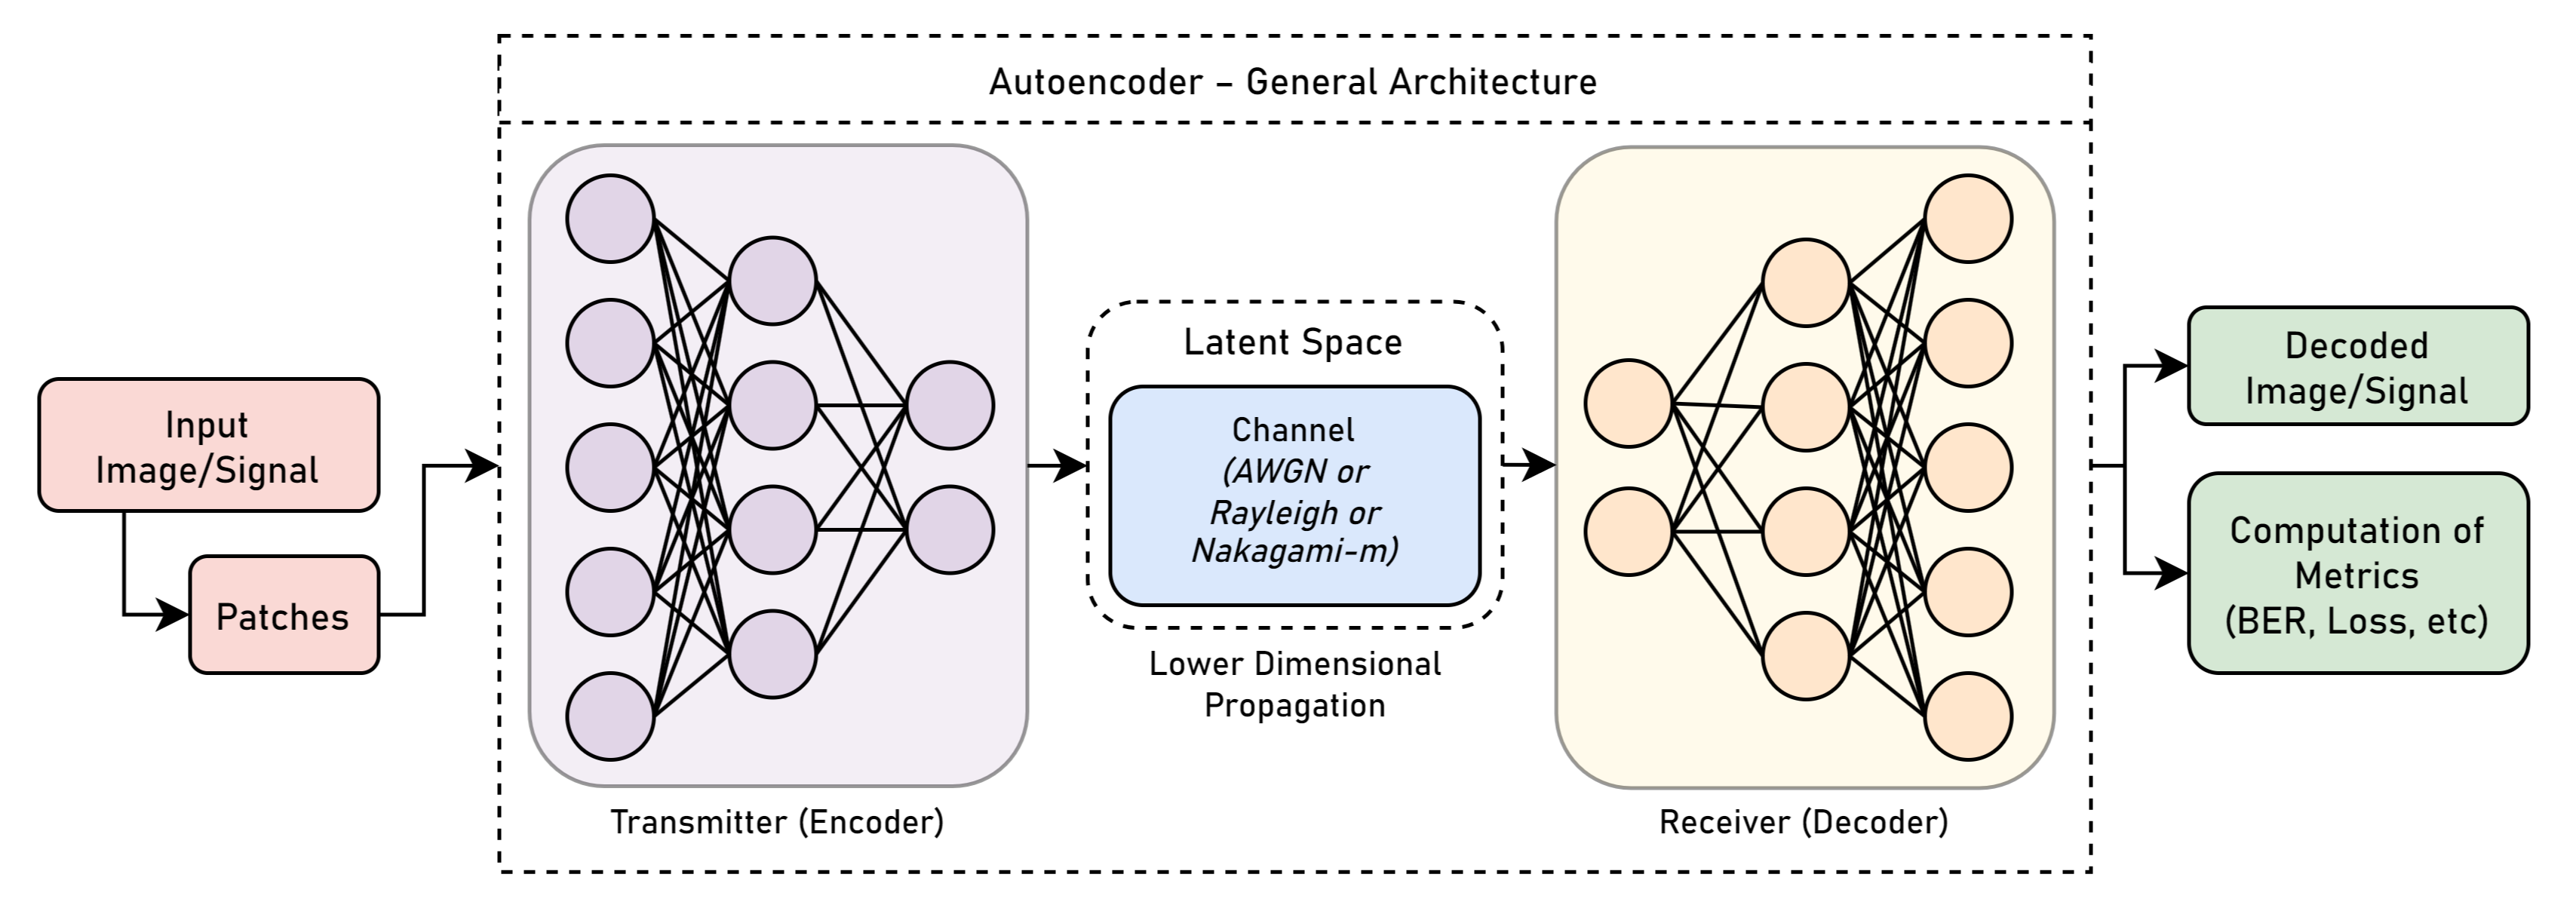
\includegraphics[width=0.8\textwidth]{figs/flow.png}
    \caption{The workflow of AeCC, demonstrating the use of autoencoders for compressed communication.}
    \label{fig:Workflow}
\end{figure*}
\begin{figure*}[b!]
    \centering
    \includegraphics[width=0.8\textwidth]{figs/batch.pdf}
    \caption{A sample of batch images used for model training.}
    \label{fig:batch}
\end{figure*}

\section{Methodology}
This section outlines the comprehensive methodology adopted for the development and experimentation of the Denoising AutoEncoder Vision Transformer (DAE-ViT) models \ref{fig:Workflow}. Our approach integrates the Vision Transformer (ViT) architecture with a denoising autoencoder to explore its potential in image processing tasks. The key contributions involve the creation of ViT models of varying sizes, training on diverse datasets, incorporation of denoising techniques, and the utilization of IEEE 754 for feature representation.

\subsection{Datasets}
To evaluate the proposed DAE-ViT models comprehensively, we employed three distinct datasets for training the Vision Transformer models:
\begin{itemize}
    \item \textbf{CIFAR-10}The CIFAR-10 dataset, consisting of 60,000 32x32 color images across ten different classes, was used for training the initial ViT models.
    \item \textbf{CIFAR-100}CIFAR-100, an extension of CIFAR-10, contains 100 classes with 600 images each. This dataset offers a more challenging environment for evaluating the robustness and generalization capabilities of the DAE-ViT models.
    \item \textbf{ImageNet}ImageNet, a large-scale dataset with over a million images across 1,000 classes, was employed to assess the scalability and performance of the proposed models on more complex and diverse visual recognition tasks \ref{fig:batch}.
\end{itemize}

\subsection{Vision Transformer Models}
To explore the impact of model size on performance, we instantiated ViT models of varying dimensions, namely ViT Tiny, ViT Small, and ViT Large. The sizes of these models were configured based on parameters such as patch size, embedding dimension, and the number of transformer layers and heads.
\begin{enumerate}
    \item \texttt{vit\_tiny = ViTModel(patch\_size=16, emb\_dim=192, num\_layers=6, num\_heads=3)}
    \item \texttt{vit\_small = ViTModel(patch\_size=16, emb\_dim=384, num\_layers=12, num\_heads=6)}
    \item \texttt{vit\_large = ViTModel(patch\_size=16, emb\_dim=768, num\_layers=24, num\_heads=12)}
\end{enumerate}

\subsection{DAE-ViT Training}
\begin{itemize}
    \item \textbf{ViT Tiny Autoencoder}The DAE-ViT model was instantiated using the ViT Tiny configuration as the base. During training, the CIFAR-10 and CIFAR-100 datasets were utilized to fine-tune the model parameters, leveraging PyTorch and PyTorch Lightning.
    \item \textbf{ Latent Space and Rayleigh Noise}Once the images passed through the latent space of the ViT Tiny autoencoder, Rayleigh noise was introduced to enhance the model's robustness. The Rayleigh Channel was employed to add noise to the lower-dimensional representation.
    \item \textbf{ Feature to Bit Conversion}For ViT Small, the 192 features obtained from the model were converted to bits using the IEEE 754 floating-point converter. This process involved the utilization of the provided helper functions for float-to-binary and binary-to-float conversions.
\end{itemize}

\begin{figure}[t!]
    \centering
    \includegraphics[width=0.375\textwidth]{figs/rbpsk.pdf}
    \caption{A visualization of the received noisy points in the data.}
    \label{fig:Noisy}
\end{figure}

\subsection{Model Averaging with EMA}
To stabilize the training process and improve model generalization, Exponential Moving Average (EMA) was implemented. This technique involves maintaining a moving average of model weights during training. Several utility functions were incorporated to streamline the training process and enhance the efficiency of the PyTorch Lightning framework. These utilities include customized progress bars, data preprocessing functions, and mean and standard deviation calculations.

\begin{figure}[b!]
    \centering
    \includegraphics[width=0.44\textwidth]{figs/umap_features.pdf}
    \caption{UMAP visualization of the encoded features (left) and channel-impaired features (right) in the feature space.}
    \label{fig:features}
\end{figure}

\section{Results \& Evaluation}
\subsection{Constellation Diagram}
Firstly, we generate a constellation diagram to visually represent the transmission of information through a communication system. It begins by instantiating a Binary Phase Shift Keying (BPSK) transmitter and an IEEE 754 converter for single precision. The encoded data is converted to a binary representation and then modulated using BPSK. Unique modulation symbols are extracted, and a scatter plot is created to depict these symbols in the complex plane.

\begin{figure*}[t!]
    \centering
    \includegraphics[width=0.65\textwidth]{figs/comparison.pdf}
    \caption{Comparison of original and reconstructed images under wireless fading conditions.}
    \label{fig:reconstructed}
\end{figure*}

\subsection{Received Noisy Signals}
Then we introduce complex noise to the previously generated constellation diagram to simulate the impact of noise in a communication channel. A noise addition function is defined, and a noise factor (fct) is set to control the level of noise. The modulated symbols are split into two arrays based on their sign, and noise is independently added to each array. The resulting noisy modulated arrays are then plotted alongside the noiseless constellation diagram. The points with positive and negative values are visualized in distinct colors, green and blue respectively, to represent the received signals. The scatter plot showcases the effect of noise on the transmitted symbols, providing a comparative view of the noiseless and noisy constellations as in \ref{fig:Noisy}.

\subsection{Features with Noise}
Then we illustrate the process of obtaining noisy feature vectors through the use of UMAP (Uniform Manifold Approximation and Projection). Initially, the feature vectors (encoded) and their noisy counterparts (encoded\_noise) are flattened to facilitate visualization. Subsequently, UMAP is applied to both sets of flattened feature vectors, producing two-dimensional representations (umap\_encoded and umap\_encoded\_noise). The UMAP-encoded features are then visualized using a scatter plot with two subplots. The left subplot represents the UMAP-encoded features without noise, depicted in light pink, while the right subplot portrays the UMAP-encoded features with added impairment, displayed in light cyan.The visualization offers insights into how noise affects the distribution and structure of the feature vectors in the reduced-dimensional space as in \ref{fig:features}.

\subsection{Reconstructed Image}
The decoding and reconstruction process involves taking the received image, which has undergone transmission and potentially been affected by noise, and reconstructing it through the Vision Transformer (ViT) model. The received image is initially flattened, transforming it into a one-dimensional array. Subsequently, this flattened representation is decoded using the ViT decoder, which involves applying linear transformations and rearranging the data to restore its original structure. The resulting decoded features are then reshaped back into a two-dimensional format, resembling the dimensions of the original image. This reconstructed image, obtained through the ViT decoding process, serves as an approximation of the transmitted image, even in the presence of noise, allowing for an evaluation of the model's robustness and the effectiveness of the decoding mechanism as shown in \ref{fig:reconstructed}.

\subsection{Training and Validation Loss}
The training and validation loss metrics serve as crucial indicators during the training phase of a machine learning model, such as the Vision Transformer (ViT) in this context. The training loss is a measure of how well the model is performing on the training dataset. It quantifies the difference between the predicted outputs of the model and the actual ground truth labels for the training samples. The goal during training is to minimize this loss, which is typically achieved through optimization algorithms, such as stochastic gradient descent (SGD), that adjust the model parameters based on the computed gradients as expressed in \ref{fig:loss}.It was trained using MSE which is given as:
\begin{equation}
    \text{MSE} = \frac{1}{N} \sum_{i=1}^{N} (y_i - \hat{y}_i)^2,z,
\end{equation}
where \(N\) is the total number of samples, \(y_i\) represents the ground truth (target) for the \(i\)-th sample, and \(\hat{y}_i\) is the predicted value for the \(i\)-th sample.

On the other hand, the validation loss is computed on a separate dataset, namely the validation set, which the model has not seen during training. The validation set serves as an independent measure of the model's generalization performance. Monitoring the validation loss helps prevent overfitting, a condition where the model learns to perform well on the training data but struggles to generalize to new, unseen data. The ideal scenario is to achieve low training and validation losses simultaneously, indicating that the model is learning the underlying patterns in the data without overfitting.

In summary, the training loss guides the optimization process during training, while the validation loss provides an external measure of the model's performance on unseen data, assisting in the evaluation of its generalization capabilities.
\begin{figure}[t!]
    \centering
    \includegraphics[width=0.44\textwidth]{figs/psnr.pdf}
    \caption{Peak Signal to Noise Ratio (PSNR) for images received under channel imapirments.}
    \label{fig:psnr}
\end{figure}

\subsection{Structural Similarity Index}
The Structural Similarity Index (SSIM) is a metric used to quantify the structural similarity between two images. In the context of the encoded and decoded images generated by the Vision Transformer (ViT), the SSIM is employed to assess how closely the reconstructed images resemble the original encoded representations as shown in \ref{fig:ssi}.
The formula for SSIM is given by:
\[
    \text{SSIM}(x, y) = \frac{(2\mu_x\mu_y + C_1)(2\sigma_{xy} + C_2)}{(\mu_x^2 + \mu_y^2 + C_1)(\sigma_x^2 + \sigma_y^2 + C_2)},
\]
where \(x\) and \(y\) are the compared images, \(\mu_x\) and \(\mu_y\) are the means, \(\sigma_x\) and \(\sigma_y\) are the standard deviations, and \(\sigma_{xy}\) is the covariance of \(x\) and \(y\), respectively. Further, \(C_1\) and \(C_2\) are small constants to avoid instability issues.

For this application, the SSIM is calculated by comparing the luminance, contrast, and structure of the encoded images with their corresponding decoded counterparts. A higher SSIM value, ranging from -1 to 1, indicates a greater similarity between the two images, with 1 representing a perfect match. Conversely, a lower SSIM value suggests more dissimilarity.

The SSIM is a valuable metric in image processing and computer vision tasks, providing insights into the fidelity of the reconstructed images. A high SSIM suggests that the ViT model has successfully preserved the essential structural features during the encoding and decoding process, indicating the effectiveness of the model in retaining image details. Conversely, a lower SSIM may indicate potential information loss or distortion in the reconstruction.

In summary, the Structural Similarity Index is a quantitative measure employed to evaluate the similarity between the encoded and decoded images generated by the ViT model, offering valuable insights into the quality of the reconstruction process.

\begin{figure}[t!]
    \centering
    \includegraphics[width=0.445\textwidth]{figs/ssim.pdf}
    \caption{Structural Similarity Index (SSIM) scores for images received under channel impairments.}
    \label{fig:ssi}
\end{figure}

\begin{figure*}[t!]
    \centering
    \includegraphics[width=0.8\textwidth]{figs/loss.pdf}
    \caption{Graph showing the progression of training and validation loss for the AeCC model over multiple steps.}
    \label{fig:loss}
\end{figure*}
\subsection{Peak Signal to noise ratio}
Peak Signal-to-Noise Ratio (PSNR) is a widely used metric to evaluate the quality of reconstructed or compressed images. It measures the level of noise and distortion in comparison to the original, noise-free image. In the context of the encoded and decoded images generated by the Vision Transformer (ViT), PSNR provides a quantitative measure of the fidelity of the reconstruction as shown in \ref{fig:psnr}.

PSNR is calculated using the mean squared error (MSE) between the original and reconstructed images. The PSNR formula is defined as:
\[
    \text{PSNR} = 10 \cdot \log_{10}\left(\frac{\text{MAX}^2}{\text{MSE}}\right)
\]
where MAX represents the maximum possible pixel value of the image, and MSE is the mean squared error between the original and reconstructed images.

A higher PSNR value indicates a smaller amount of noise and distortion in the reconstructed image, signifying a better quality of reconstruction. Conversely, a lower PSNR suggests a higher level of distortion, indicating a significant deviation of the reconstructed image from the original.

In the case of ViT-encoded images, a higher PSNR implies that the ViT model has effectively preserved the details of the original images during the encoding and decoding process. PSNR serves as a valuable metric in image processing, offering a straightforward way to quantify the quality of image reconstruction by considering both fidelity and perceptual aspects of the reconstructed images.

\section{Conclusion}
In this research, we delved into the adaptation of Vision Transformer (ViT) models for image denoising, introducing a Denoising Autoencoder (DAEViT). Our experiments spanned diverse datasets – CIFAR-10, CIFAR-100, and ImageNet – training ViT models of different sizes, from vit\_tiny to vit\_large. The core denoising strategy involved a ViT-based autoencoder, DAEViT, which effectively reduced noise in images. Our models demonstrated robust performance across datasets, showcasing the potential of ViT in denoising tasks. We introduced Rayleigh noise to simulate real-world distortions, and IEEE 754 conversion of latent features offered insights into information preservation. In conclusion, our work establishes ViT's viability for image denoising, emphasizing its adaptability and promising denoising performance. This research contributes to the exploration of Vision Transformers in diverse computer vision applications, extending beyond conventional image classification.

\bibliographystyle{ieeetr}
\bibliography{refs}

\end{document}